\documentclass[11pt]{article}

\usepackage{graphics}
\usepackage[dvips]{graphicx}
\usepackage[left]{lineno}
\usepackage{multicol}
%\usepackage[a4paper,left=1.4cm,right=1.5cm,top=1.5cm]{geometry}
\pagenumbering{arabic}
\usepackage[utf8]{inputenc}
\setcounter{page}{01}
\usepackage[british]{babel}
\usepackage{amsmath}
\usepackage{esvect}
\usepackage{mathrsfs}  
\usepackage{amsfonts}
\usepackage[]{algorithm}
\usepackage{algpseudocode}
\usepackage[font=footnotesize,labelfont=bf]{caption}
\usepackage[font=footnotesize,labelfont=bf]{subcaption}
\usepackage{lipsum}
\usepackage[usenames, dvipsnames]{color}
\usepackage{authblk}
\usepackage{scrextend}


\title{\bf Contrast Enhancement of Color Images using a Multi-Objective Optimization Framework}
\author[1]{Luis G. Moré}
\author[1]{Diego P. Pinto-Roa}
\author[1,2]{José Luis Vázquez Noguera}
\affil[1]{Facultad Politécnica - Universidad Nacional de Asunción}
\affil[2]{Universidad Americana del Paraguay}
\affil[ ]{\textit {\{lmore,dpinto,jlvazquez\}@pol.una.py}}
\date{}                     %% if you don't need date to appear
\setcounter{Maxaffil}{0}
\renewcommand\Affilfont{\itshape\small}

\begin{document}
\maketitle
%\pagestyle{myheadings}
%\markright{\footnotesize {doi:10.6062/jcis.2015.06.01.0091 \hspace{3.5cm} Dantas et al.}}  % para book, report article

%\pagestyle{myheadings}
%\markright{\footnotesize {doi:10.6062/jcis.2015.**.**.**** %\hspace{3.5cm} Rosa et al.}}  % para book, report article
%\linenumbers
\pagenumbering{gobble}


%\includegraphics[height=1.96cm]{headP96.png}
% \vspace{1.2cm}


% \begin{center}
% %======
% %Title
% %======

% %{\bf  {\Large Contrast Enhancement of Color Images using a Multi-Objective Optimization Framework}}
% % \bigskip

% %============================
% %List of Authors and Address
% %============================

% % {\small Luis G. Moré\footnote{E-mail Corresponding Author: lmore@pol.una.py}, Diego P. Pinto-Roa, José L. Vázquez N.
% % }
% % \smallskip

% % {\small

% % }


% %{\footnotesize Received on January 01, 2015 / accepted on *****, 2015}

% \end{center}

% \quad

%============================
%Abstract and Keywords
%============================
%\hline
%\cline{5cm}
\noindent
\begin{addmargin}[2.5em]{2.5em}
\textbf{Abstract.} \small{Contrast Enhancement(CE) is a fundamental preprocessing step for several applications, and also for further decision making processes related. This task has been addressed successfully for gray-scale images using pure Multi-Objective Optimization(MOO); nevertheless, difficulties arise when performing MOO for color images. This paper presents a pure MOO approach with automatic CE for color images, taking into account evaluation metrics better suited for color spaces, which are designed to achieve the improvement in contrast and also control the noise introduced because of the contrast variation seen during the process. A series of experiments were conducted in order to assess the correctness of this approach, and the results consist of a set of contrast enhanced images, with different compromise rates between contrast modification and noise introduction. It appears that the results obtained are promising, and the numeric values of the optimization metrics are analyzed using correlation tables and discussed using the Pareto Front obtained from these values.
}

\quad

{\footnotesize
{\bf Keywords}: Multi-Objective optimization, Contrast Enhancement, MOPSO, CLAHE, Color Spaces.}


\end{addmargin}
% \begin{abstract}

% \end{abstract}

\section{Introduction}

Contrast Enhancement (CE) is a fundamental preprocessing step for several image processing applications such as Medical Imaging (Computer Aided Diagnosis \cite{doi2007computer}, Computerized Tomography Imaging \cite{kak2001principles}, Magnetic Resonance Imaging \cite{doi:10.1056/NEJM199303113281008} and others), Remote Sensing \cite{lillesand2014remote}, and so on.

Tecniques based on Histogram Equalization have been extensively proven to be valid when addressing CE problems \cite{Gonzalez02a,pizer1987adaptive,zuiderveld1994contrast,580378}. Meta-Heuristics such as Mono-Objective Optimization, and also Multi-Objective Optimization (MOO) have been tested successfully in order to solve CE problems on gray-scaled images \cite{morepso,more2015parameter,812529,HOSEINI2013879}. However, MOO applied to color images poses additional difficulties because it is neccesary to preserve color information present therein.%However, when dealing with color images, it is neccesary to take into account color spaces in which they are represented, as well as the intensity channel (in order to maximize information) and also the color channels (because preserving color information is required) which poses a challenging problem when addressing CE as a MOO problem.

Our proposal consist in testing images transformed from $RGB$ color space to $YCbCr$ in order to perform MMO-based CE. Contrast Limited Adaptive Histogram Equialization (CLAHE) is applied over the $Y$ channel of the test image in order to modify contrast, and the resultant image is transformed back to $RGB$ in order to evaluate the similarity between color channels.

The rest of the paper is organized as follows: in Section \ref{sec:theorethical_framework}, the fundametal concepts for this work are presented, in Section \ref{sec:proposal} the CE problem is posed, and our approach is presented, in Section \ref{sec:results_discussion} the results achieved are discussed in detail, and finally in \ref{sec:conclusion} some final points are remarked.

\section{Theorethical Framework}\label{sec:theorethical_framework}

This sections presents a brief introduction of the concepts used in the paper.
%The solution proposed in this paper is based in the following concepts, which are to be described briefly below. It is fundamental to explain the color spaces, the meta-heuristic and the metrics adopted in this approach.

\subsection{Color Spaces Adopted}\label{sec:color_spaces}

Original images are represented using the $RGB$ color space \cite{gonzalez2002processing}, which is a $N \times M \times 3$  array of color pixels. Every color pixel is represented by an element $[\begin{matrix}z_r & z_g & z_b\end{matrix}]$ of the array previously mentioned, where $z_r, z_g, z_b$ are the red, green, and blue components of the color pixel in a specific location. Original images are then transformed to the $YCbCr$ color space \cite{gonzalez2002processing}, which is a representation widely used in digital video. The main advantage is that the $Y$ component here represents the luminance information of the image, meanwhile the $Cb$ component represents a difference between the blue component and a reference value, and the $Cr$ component is the difference between the red component and a reference value. Another important advantage of this representation is that the conversion from $RGB$, and back to $RGB$ is straightforward:



\begin{equation}
\begin{bmatrix}
    Y \\
    C_b \\
    C_r 
\end{bmatrix} =
 \begin{bmatrix}
    16  \\
    128 \\
    128
\end{bmatrix}
+
 \begin{bmatrix}
    65.481 & 128.553 & 24.966 \\
    -37.797 & -74.203 & 112.000 \\
    112.000 & -93.786 & -18.214 
\end{bmatrix}
\begin{bmatrix}
   R \\
   G \\
   B 
\end{bmatrix}
\end{equation}
\begin{equation}
\begin{bmatrix}
    R \\
    G \\
    B 
\end{bmatrix} =
 \begin{bmatrix}
    Y + 1.402 \cdot (C_r - 128) \\
    Y -0.34414 \cdot (C_b - 128) - 0.71414 \cdot (C_r - 128) \\
    Y + 1.772 \cdot  (C_b - 128) 
\end{bmatrix}
\end{equation}

\subsection{Contrast Limited Adaptive Histogram Equalization (CLAHE)}

Contrast Limited Adaptive Histogram Equalization (CLAHE) \cite{zuiderveld1994contrast} is a well known CE algorithm, designed for broad applicability in the context of digital image proccessing. CLAHE is a variation of the \textit{Adaptive Histogram Equalization (AHE)}\cite{pizer1987adaptive} CE algorithm. In AHE, an image is processed transforming each pixel using a function based on the histogram of its surrounding pixels, defined by a \textit{Contextual Region $(\mathscr{R}_x,\mathscr{R}_y)$}. CLAHE limits the CE by clipping the resultant histogram based in a coefficient called \textit{Clip Limit} $\mathscr{C}$

\subsection{Multi-Objective Particle Swarm Optimization (MOPSO)}

Multi-Objective Particle Swarm Optimization ($MOPSO$) \cite{nebro2009smpso} is a widely known metaheuristic algorithm. It is a bio-inspired metaheuristic which mimics the social behavior of bird flocking. In $PSO$, every potential solution of the problem being approached is called a \textit{particle} and the actual population of solutions is called a \textit{swarm}. Every particle $\vv{x}$ performs a search within a search space $\Omega$, and for every generation $t$, every solution $\vv{x}$ is updated according to:

\begin{equation}\label{eq:posicion1}
\vv{x}_i(t) = \vv{x}_i(t-1) + \vv{v}_i(t)
\end{equation}

Here, $\vv{v}$ is a factor known as the velocity, and is given by:

\begin{equation}\label{eq:velocidad1}
 \vv{v}_i(t) = w \cdot (t-1) + C_1 \cdot r_1 \cdot (\vv{x}_{p_i} - \vv{x}_i) + C_2 \cdot r_2 \cdot (\vv{x}_{g_i} - \vv{x_i}) \text{,}
\end{equation}
where $\vv{x}_{p_i}$ is the best solution that $\vv{x}_i$ has found so far, $\vv{x}_{g_i}$ is the best solution that the entire swarm has found at the current iteration, $w$ is a coeficient known as the \textit{inertia weight}, which controls the search speed rate of $PSO$; $r_1$ and $r_2$ are random numbers between $[0,1]$. Finally, $C_1$ and $C_2$ are coefficient which control the weight between global and local particles during the search.

In $MOPSO$, a \textit{constriction coefficient} $\chi$ is adopted in order to control the particle's velocity, as described below:

\begin{equation}
\chi = \frac{2}{2 - \varphi - \sqrt{\varphi^2 - 4 \varphi}}
\end{equation}

where

\begin{equation}
% \[
    \varphi= 
\begin{cases}
    C_1 + C_2 & \text{if } C_1 + C_2 > 4\\
    0,              & \text{if } C_1 + C_2 \leq 4
\end{cases}
% \]
\end{equation}

Furthermore, the velocity in $MOPSO$ is bounded by the following \textit{velocity constriction} equation:
\begin{equation}\label{eq:restricciondelta}
% \[
v_{i,j}(t)= 
\begin{cases}
    delta_j & \text{if } v_{i,j}(t) > delta_j\\
    -delta_j,      & \text{if } v_{i,j}(t) \leq delta_j \\
    v_{i,j}(t),      & \text{otherwise }
\end{cases}
% \]
\end{equation}

where

\begin{equation}
delta_j=\frac{upper\_limit_j - lower\_limit_j}{2}
\end{equation}


\subsection{Entropy of image}

Entropy of image \cite{108593} is a metric that measures how much information is represented within an image. Entropy and contrast are closely related to the intensity distribution of images, so this metric is able to assess contrast variations as a consecuence of image transformations.

First, we need to define the \textit{Histogram} of intensities of an image $H$ as follows: Let $c_1, c_2, ..., c_n$ the count of pixels with intensity $i_1, i_2, ..., i_n$ respectively, and also let

\begin{equation}
p_i=\frac{c_i}{N}, \qquad \sum_{i=1}^n c_i = N, \qquad i= 1,2, ..., n,
\end{equation}

where $N$ is the total sum of pixels shown in an image $I$ and $n$ is every intensity level representable by the color space of $I$. Then $H$ is defined as a probability distribution in which every $p_i$ represents the probability of occurrence of an intensity $i$. Then, Entropy of Image is defined as below:

\begin{equation}
\mathscr{H}= -\sum_{i=0}^{n-1} p_i \text{log}_2(p_i) \qquad \mathscr{H} \in \{0,...,\text{log}_2(n)\}
\end{equation}

\subsection{Structural Similarity Index}

The \textit{Structural Similarity Index} ($SSIM$) \cite{wang2004image} is a well known metric that measures important image's attributes such as \textit{Luminance, Contrast} and \textit{Structure}. SSIM main aim is to measure the distortion added to the image as a consecuence of the CE proccess. $SSIM$ is calculated by windows, so given two images $I_x$ and $T_y$ which represent an original and an enhanced image, respectively, the $SSIM$ index is defined as below:

\begin{equation}
SSIM(I,T) = \frac{(2\mu_{I_x} \mu_{T_y}+E_1)(2\sigma_{I_xT_y}+E_2)}{(\mu^2_{I_x}+\mu^2_{T_y}+E_1)(\sigma^2_{I_x} + \sigma^2_{T_y}+E_2)} \qquad SSIM \in [0,1]
\end{equation}

where $\mu_{I_x}$, $\mu_{T_y}$ is the intensity averages of $I_x$ and $T_y$, respectively; $\sigma^2_{I_x}$ and  $\sigma^2_{T_y}$ are the intensity variances for $I_x$ and $T_y$, respectively; $\sigma_{I_xT_y}$ is the covariance between $I_x$ and $T_y$ intensities. $E_1=(K_1L^2)$, where $L$ is the dynamic range of intensities of image's pixels, and $K_1 \ll 1$ is a small constant; $E_2=(K_2L)^2$, and $K_2 \ll 1$; both $E_1$ and $E_2$ are constants used to stabilize division when denominator is close to zero.

\section{Formulation of the Problem Posed}\label{sec:formulation}

Given an color input image $I$, with $M \times N$ pixels, and a vector $\vv{x}=(\mathscr{R}_x,\mathscr{R}_y,\mathscr{C})$, where $\mathscr{R}_x$ and $\mathscr{R}_y$ are contextual regions and $\mathscr{C}$ is the \textit{Clip Limit}, a set of non-dominated solutions $\mathscr{X}$, which simultaneously maximize the objective functions $f_1,f_2,f_3,f_4$:

\begin{equation}
\mathscr{F} = [f_1(I,\vv{x}),f_2(I,\vv{x}),f_3(I,\vv{x}),f_4(I,\vv{x})]; \qquad f_1,f_2,f_3,f_4 \in [0,1]
\end{equation}

where:

\begin{itemize}
	\item $T_y$ is the enhanced intensity map, when applying $\vv{x}$ to $I_y$; this is: $T_y=CLAHE(\vv{x},I_y)$. $T_y$ and $I_y$ are the $Y$ channel in the $YCbCr$ representation of $I$ and $T$, respectively,
	\item $f_1(I,\vv{x})=\frac{\mathscr{H}(T)}{\text{log}_2L}$ is the normalized Entropy of the enhanced intensity map $T_y$, as described above.
	\item $f_2(I,\vv{x})=SSIM(I_R,T_R)$ is the $SSIM$ measure between $I_R$ and $T_R$. $I_R$ and $T_R$ are the $R$ channel of the $RGB$ representation of $I$ and $T$, respectively.
	\item $f_3(I,\vv{x})=SSIM(I_G,T_G)$ is the $SSIM$ measure between $I_G$ and $T_G$. $I_G$ and $T_G$ are the $G$ channel of the $RGB$ representation of $I$ and $T$, respectively.
	\item $f_4(I,\vv{x})=SSIM(I_B,T_B)$ is the $SSIM$ measure between $I_B$ and $T_B$. $I_B$ and $T_B$ are the $B$ channel of the $RGB$ representation of $I$ and $T$, respectively.
\end{itemize}

Bounded to:

\begin{itemize}
\item $\mathscr{R}_x \in [2,...,M]$ for the $\mathbb{N}$ numbers,
\item $\mathscr{R}_y \in [2,...,N]$ for the $\mathbb{N}$ numbers,
\item $\mathscr{C} \in (0,...,1]$ for the $\mathbb{R}$ numbers.
\end{itemize}	

\section{Proposal}\label{sec:proposal}

\begin{algorithm}[H]
    \scriptsize
    \begin{algorithmic}[1]
        \Require Input image $I$, amount of particles $\Omega$, iterations $t_{max}$
        \State Initialize $\omega$, $c_1$, $c_2$, $t=0$, $lower\_limit_1$, $lower\_limit_2$, $lower\_limit_3$, $upper\_limit_1$, $upper\_limit_2$, $upper\_limit_3$, $\mathscr{X}$
        %\For{cada $i$-ésima partícula del enjambre}
        %    \State Inicializar la posición $x_i$ aleatoriamente
        %    \State Inicializar la velocidad $v_i$ a 0
        %    \State ${imagenMejorada}$ = CLAHE(${x_i}$, ${imagenOriginal}$)
        %    \State ${f_i}$ = evaluarAptitud(${imagenOriginal}$, ${imagenMejorada}$)
        %    \State Establecer el mejor individual inicial $p_i$ por el valor inicial $x_i$
        %    \If{$f_i < f_{p_g}$}
        %        \State reemplazar $p_g$ por el valor de $x_i$
        %    \EndIf
        %\EndFor
        \While{$t$ $<$ $t_{max}$}
            \For{every $i$-th particle}
                \State Calculate new velocity $\overrightarrow{v_i}^t$ of the particle  using equations \eqref{eq:velocidad1} and \eqref{eq:restricciondelta}
                \State Calculate new particle position $\overrightarrow{x_i}^t$ using expression \eqref{eq:posicion1}

                \State ${T}$ = CLAHE(${\overrightarrow{x_i}^t}$, ${I}$)
                \State ${f^t_i}$ = $f(I, \overrightarrow{x_i}^t)$%evaluarAptitud(${I}$, ${T}$) 
                \If{$ \overrightarrow{x_i} \succ \overrightarrow{x_{p_i}}$}
                    \State replace $\overrightarrow{x}_{p_i}$ by $\overrightarrow{x_i}^t$
                \EndIf
                \If{$ \overrightarrow{x_i} \succ \overrightarrow{x_{g_i}}$  }
                    \State Update the Pareto set $\mathscr{X}$
                \EndIf
                \State $t$ = $t$ + 1
            \EndFor
        \EndWhile
    \Ensure $\mathscr{X}$
    \end{algorithmic}
    \caption{MOPSO-CLAHE}
    \label{alg:pso_clahe}
\end{algorithm}

\textbf{Algorithm \ref{alg:pso_clahe}} shows how Color Multi-Objective PSO-CLAHE ($CMOPSO-CLAHE$) is implemented, in order to tune parameters of $CLAHE$. The parameters received by $CLAHE$ are stored by a particle $\vv{x}=(\mathscr{R}_x,\mathscr{Y}_x,\mathscr{C})$, the original image $I$ is transformed to its $YCrCb$ representation,and $\vv{x}$ is applied to the $Y$ channel, in order to obtain a $Y_T$ intensity map, which is used to transform back to $RGB$, to obtain the resulting image $T$. The resulting images are evaluated according to the metrics $\mathscr{H}_Y$, $SSIM_R$, $SSIM_G$, $SSIM_B$, which are the entropy of resulting images measured in the $Y$ channel of the $YCrCb$ representation of these, and $SSIM_R,SSIM_G,SSIM_B$ are the $SSIM$ measures for original and resulting images using the $R,G,B$ channels of the $RGB$ representations of these. The non-dominated solutions are then stored in the Pareto set. $CMOPSO-CLAHE$ proccess is repeated until a criterion stop is reached.


\section{Results and Discussion}\label{sec:results_discussion}

\begin{table}[H]
\setlength{\abovecaptionskip}{2pt plus 3pt minus 2pt} % Chosen fairly arbitrarily
\caption[Parámetros de entrada para $MOPSO$]{Initial parameters for CMOPSO-CLAHE.}
\begin{center}
 \begin{tabular}{||c c | c c||} 
 \hline
 Parameter & Value & Parameter & Value \\ [0.5ex] 
 \hline\hline
 $lower\_limit_{\mathscr{R}_x}$ & $2$ & $upper\_limit_{\mathscr{R}_x}$ & $M/2$ \\ 
 \hline
 $lower\_limit_{\mathscr{R}_y}$ & $2$ & $upper\_limit_{\mathscr{R}_y}$ & $N/2$ \\  
 \hline
 $lower\_limit_{{\mathscr{C}}}$ & $0$ & $upper\_limit_{{\mathscr{C}}}$ & 0.5 \\
\hline
$\Omega$ & $100$ & $t_{max}$ & $100$ \\ 
\hline
$c_1$ $min$ & 1.5 & $c_1$ $max$ & 2.5 \\ 
\hline
$c_2$ $min$ & 1.5 & $c_2$ $max$ & 2.5 \\ 
\hline
$r_1$ $min$ & 0.0 & $r_1$ $max$ & 1.0 \\ 
\hline
$r_2$ $min$ & 0.0 & $r_2$ $max$ & 1.0 \\
\hline
\end{tabular}
\end{center}
\label{table:parametrospso}
\end{table}

Tests were performed using 8 color images from the dataset available at http://www.vision.caltech.edu/archive.html. Table \ref{table:parametrospso} shows how $SMPSO$ was configured for the tests. $SMPSO$ implementation is available at \cite{durillo2010jmetal}, meanwhile the implementations for $CLAHE$, $\mathscr{H}$ and $SSIM$ are available at \cite{bradski2000opencv}. For every test image, 50 test were performed, and 10 non-dominated solutions were found in average. From Figures (\ref{fig:casa1original},\ref{fig:casa1enhanced1},\ref{fig:casa1enhanced2}) it is noticeable how CE is achieved; there is also a compromise relation between $\mathscr{H}$ and $SSIM_R,SSIM_G,SSIM_B$. It is noteworthy from Figure (\ref{fig:casa1enhanced2}) how higher values of $\mathscr{H}$ degrade images severely, so it is neccesary to find the correct balance between $\mathscr{H}$ and $SSIM_R,SSIM_G,SSIM_B$. In Figure (\ref{fig:casa1enhanced3}) it is shown the resultant image enhanced using the proposal described in \cite{morepso}; it is noticeable that the resultant image does not achieve good CE; this is because the mono-objective approach does not use color information properly, and this result is the same for other test images. In Table \ref{table:nodominadas}, the non-dominated metric coefficients are shown, and in the last line it is shown the metric coefficients for image (\ref{fig:casa1original}), enhanced using the mono-objective proposal. Although its metrics seem to fall in the Pareto Front, the visual information obtained is not enough to state that the mono-objective proposal is feasible for color images. These results are similar for every test image used.

% \begin{figure}[htp]

% \centering
% 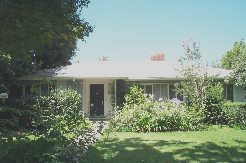
\includegraphics[width=.3\textwidth]{calhouse_0230.jpg}\hfill
% 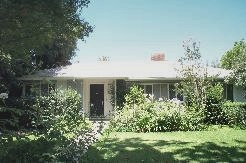
\includegraphics[width=.3\textwidth]{calhouse_0230_20-25165283474-10.jpg}\hfill
% 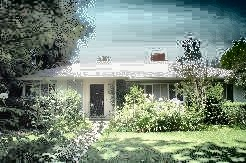
\includegraphics[width=.3\textwidth]{calhouse_0230_20-62968204656-00.jpg}

% \caption{default}
% \label{fig:figure3}

% \end{figure}

\begin{figure}[H]
    \centering
    \begin{subfigure}[t]{0.45\textwidth}
        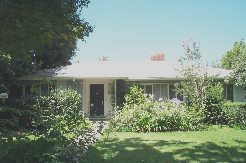
\includegraphics[width=\textwidth]{calhouse_0230.jpg}
        \caption{Original Image. $\mathscr{H_Y}=0.207231$, $SSIM_R=1$, $SSIM_G=1$, $SSIM_B=1$}
        \label{fig:casa1original}
    \end{subfigure}
    ~ %add desired spacing between images, e. g. ~, \quad, \qquad, \hfill etc. 
      %(or a blank line to force the subfigure onto a new line)
    \begin{subfigure}[t]{0.45\textwidth}
        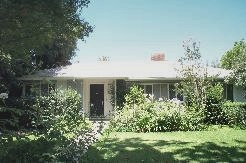
\includegraphics[width=\textwidth]{calhouse_0230_20-25165283474-10.jpg}
        \caption{Enhanced Image. $\mathscr{H_Y}=0.611275$, $SSIM_R=0.00897331$, $SSIM_G=0.00823064$, $SSIM_B=0.00851013$}
        \label{fig:casa1enhanced1}
    \end{subfigure} \\
    ~ %add desired spacing between images, e. g. ~, \quad, \qquad, \hfill etc. 
    %(or a blank line to force the subfigure onto a new line)
    \begin{subfigure}[t]{0.45\textwidth}
        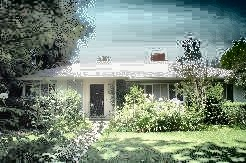
\includegraphics[width=\textwidth]{calhouse_0230_20-62968204656-00.jpg}
        \caption{Enhanced Image.  $\mathscr{H_Y}=0.0350595$, $SSIM_R=0.416776$, $SSIM_G=0.403636$, $SSIM_B=0.417654$}
        \label{fig:casa1enhanced2}
    \end{subfigure} 
    \begin{subfigure}[t]{0.45\textwidth}
        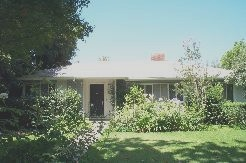
\includegraphics[width=\textwidth]{calhouse_0230_20-20-0020072469292179818.jpg}
        \caption{Enhanced Image using \cite{morepso}. $\mathscr{H_Y}=0.788927$, $SSIM_R=0.000204143$, $SSIM_G=0.0000526475$, $SSIM_B=0.0000518143$}
        \label{fig:casa1enhanced3}
    \end{subfigure}

    \caption{Original and resultant images of House 1}\label{fig:casa1}
\end{figure}

\begin{table}[H]
\setlength{\abovecaptionskip}{2pt plus 3pt minus 2pt} % Chosen fairly arbitrarily
\caption[Parámetros de entrada para $MOPSO$]{Correlation table between metrics. Data was taken from Table \ref{table:nodominadas}.}
\begin{center}
 \begin{tabular}{||c | c c c c||} 
 \hline
Metrics & $\mathscr{H_Y}$ & $SSIM_R$ & $SSIM_G$ & $SSIM_B$ \\ 
\hline
$\mathscr{H_Y}$ & 1 &   &   &  \\ 
\hline
$SSIM_R$ & -0.9826  & 1 &  &  \\ 
\hline
$SSIM_G$ & -0.9823 & 0.9999   & 1   &  \\ 
\hline
$SSIM_B$ & -0.9826 & 0.9999   & 0.9999   & 1 \\ 
\hline
\end{tabular}
\end{center}
\label{table:correlacion}
\end{table}


\begin{table}[H]
\setlength{\abovecaptionskip}{2pt plus 3pt minus 2pt} % Chosen fairly arbitrarily
\caption[Parámetros de entrada para $MOPSO$]{Metric coefficients obtained using our approach for some non-dominated results from image in Figure (\ref{fig:casa1}), and the coefficients obtained using the approach of \cite{morepso}, shown in the last line.}
\begin{center}
\resizebox{0.8\columnwidth}{!}{%
 \begin{tabular}{||c | c c c c||} 
 \hline
 & $\mathscr{H_Y}$ & $SSIM_R$ & $SSIM_G$ & $SSIM_B$ \\ 
\hline
Result 1 & 0.544854	& 0.0155038	 & 0.0140995  & 0.0149364 \\ 
\hline
Result 2& 0.658577	& 0.00551113 & 0.00494194 & 0.00529456 \\ 
\hline
Result 3& 0.0425715	& 0.394656	 & 0.380667	  & 0.39842 \\ 
\hline
Result 4& 0.0365424	& 0.401675	 & 0.388628	  & 0.402692 \\ 
\hline
Result 5& 0.0350595	& 0.416776	 & 0.403636	  & 0.417654 \\ 
\hline
Result 6& 0.611275	& 0.00897331 & 0.00823064 & 0.00851013 \\ 
\hline
Result 7& 0.0342894	& 0.420948	 & 0.408035	  & 0.421891 \\ 
\hline
Result Mono& 0.788927    & 0.000204143 & 0.0000526475 & 0.0000518143 \\
\hline
\end{tabular}
}
\end{center}
\label{table:nodominadas}
\end{table}


\begin{figure}[H]
    \centering
        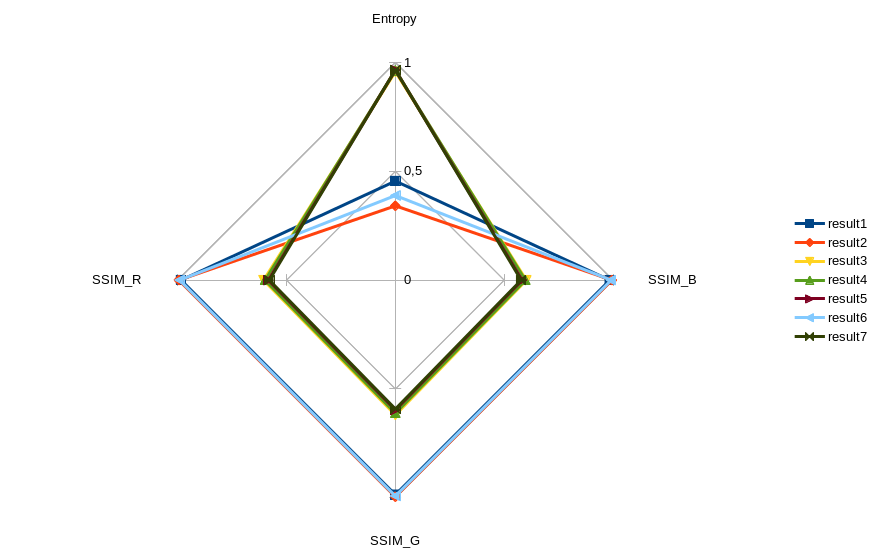
\includegraphics[width=0.80\textwidth]{pareto_front.png}
    \caption{Pareto front drawed using data from Table \ref{table:nodominadas} }\label{fig:pareto_front}
\end{figure}



Figure (\ref{fig:pareto_front}) shows the Pareto Front created from the data in Table \ref{table:nodominadas}, and also Table \ref{table:correlacion} shows the correlation between metrics, analized from the results in Table \ref{table:nodominadas}. It is remarkable that there is a strong positive correlation between $SSIM_R$, $SSIM_G$ and $SSIM_B$; and there is a negative correlation between the previously mentioned metrics and $\mathscr{H_Y}$. These correlations indicate that the channels $R,G,B$ of images are directly affected by the proccess that modifies $Y$ channel (see Algorithm (\ref{alg:pso_clahe})). This also indicates that CE of color images can be posed as a bi-objective optimization problem, using only $\mathscr{H_Y}$ and $SSIM$ applied over $Y$ channel.

\section{Conclusion}\label{sec:conclusion}

A Multi-Objective approach for Contrast Enhancement of color images is presented, which takes into account intensity and color information as Multi-Objective metrics. This approach achieves several resultant images, with different compromise rates between contrast and structural-similarity, in order to maximize information available for further analysis.

The authors are still performing test with similar images found in the database. As future work, it would be useful to analyse the parameters used for the meta-heuristics, the use of non-marginal metrics to assess the resultant images obtained with the approach, and perform tests posing CE of color images as a bi-objective optimization problem. 

\bibliographystyle{unsrt}
\bibliography{bibliografia}

\end{document}
